% Options for packages loaded elsewhere
% Options for packages loaded elsewhere
\PassOptionsToPackage{unicode}{hyperref}
\PassOptionsToPackage{hyphens}{url}
\PassOptionsToPackage{dvipsnames,svgnames,x11names}{xcolor}
%
\documentclass[
  10pt,
  letterpaper,
  DIV=11,
  numbers=noendperiod]{scrartcl}
\usepackage{xcolor}
\usepackage{amsmath,amssymb}
\setcounter{secnumdepth}{5}
\usepackage{iftex}
\ifPDFTeX
  \usepackage[T1]{fontenc}
  \usepackage[utf8]{inputenc}
  \usepackage{textcomp} % provide euro and other symbols
\else % if luatex or xetex
  \usepackage{unicode-math} % this also loads fontspec
  \defaultfontfeatures{Scale=MatchLowercase}
  \defaultfontfeatures[\rmfamily]{Ligatures=TeX,Scale=1}
\fi
\usepackage{lmodern}
\ifPDFTeX\else
  % xetex/luatex font selection
\fi
% Use upquote if available, for straight quotes in verbatim environments
\IfFileExists{upquote.sty}{\usepackage{upquote}}{}
\IfFileExists{microtype.sty}{% use microtype if available
  \usepackage[]{microtype}
  \UseMicrotypeSet[protrusion]{basicmath} % disable protrusion for tt fonts
}{}
% Make \paragraph and \subparagraph free-standing
\makeatletter
\ifx\paragraph\undefined\else
  \let\oldparagraph\paragraph
  \renewcommand{\paragraph}{
    \@ifstar
      \xxxParagraphStar
      \xxxParagraphNoStar
  }
  \newcommand{\xxxParagraphStar}[1]{\oldparagraph*{#1}\mbox{}}
  \newcommand{\xxxParagraphNoStar}[1]{\oldparagraph{#1}\mbox{}}
\fi
\ifx\subparagraph\undefined\else
  \let\oldsubparagraph\subparagraph
  \renewcommand{\subparagraph}{
    \@ifstar
      \xxxSubParagraphStar
      \xxxSubParagraphNoStar
  }
  \newcommand{\xxxSubParagraphStar}[1]{\oldsubparagraph*{#1}\mbox{}}
  \newcommand{\xxxSubParagraphNoStar}[1]{\oldsubparagraph{#1}\mbox{}}
\fi
\makeatother


\usepackage{longtable,booktabs,array}
\usepackage{calc} % for calculating minipage widths
% Correct order of tables after \paragraph or \subparagraph
\usepackage{etoolbox}
\makeatletter
\patchcmd\longtable{\par}{\if@noskipsec\mbox{}\fi\par}{}{}
\makeatother
% Allow footnotes in longtable head/foot
\IfFileExists{footnotehyper.sty}{\usepackage{footnotehyper}}{\usepackage{footnote}}
\makesavenoteenv{longtable}
\usepackage{graphicx}
\makeatletter
\newsavebox\pandoc@box
\newcommand*\pandocbounded[1]{% scales image to fit in text height/width
  \sbox\pandoc@box{#1}%
  \Gscale@div\@tempa{\textheight}{\dimexpr\ht\pandoc@box+\dp\pandoc@box\relax}%
  \Gscale@div\@tempb{\linewidth}{\wd\pandoc@box}%
  \ifdim\@tempb\p@<\@tempa\p@\let\@tempa\@tempb\fi% select the smaller of both
  \ifdim\@tempa\p@<\p@\scalebox{\@tempa}{\usebox\pandoc@box}%
  \else\usebox{\pandoc@box}%
  \fi%
}
% Set default figure placement to htbp
\def\fps@figure{htbp}
\makeatother





\setlength{\emergencystretch}{3em} % prevent overfull lines

\providecommand{\tightlist}{%
  \setlength{\itemsep}{0pt}\setlength{\parskip}{0pt}}



 


\usepackage{booktabs}
\usepackage{caption}
\usepackage{longtable}
\usepackage{colortbl}
\usepackage{array}
\usepackage{anyfontsize}
\usepackage{multirow}
\usepackage{xcolor, soul}
\definecolor{Light}{gray}{.90}
\sethlcolor{Light}
\let\OldTexttt\texttt
\renewcommand{\texttt}[1]{\OldTexttt{\hl{#1}}}
\usepackage{caption}
\captionsetup{font=small, labelfont=bf}
\setlength{\parindent}{0pt}
\setlength{\parskip}{1.25ex}
\KOMAoption{captions}{tableheading}
\makeatletter
\@ifpackageloaded{caption}{}{\usepackage{caption}}
\AtBeginDocument{%
\ifdefined\contentsname
  \renewcommand*\contentsname{Table of contents}
\else
  \newcommand\contentsname{Table of contents}
\fi
\ifdefined\listfigurename
  \renewcommand*\listfigurename{List of Figures}
\else
  \newcommand\listfigurename{List of Figures}
\fi
\ifdefined\listtablename
  \renewcommand*\listtablename{List of Tables}
\else
  \newcommand\listtablename{List of Tables}
\fi
\ifdefined\figurename
  \renewcommand*\figurename{Figure}
\else
  \newcommand\figurename{Figure}
\fi
\ifdefined\tablename
  \renewcommand*\tablename{Table}
\else
  \newcommand\tablename{Table}
\fi
}
\@ifpackageloaded{float}{}{\usepackage{float}}
\floatstyle{ruled}
\@ifundefined{c@chapter}{\newfloat{codelisting}{h}{lop}}{\newfloat{codelisting}{h}{lop}[chapter]}
\floatname{codelisting}{Listing}
\newcommand*\listoflistings{\listof{codelisting}{List of Listings}}
\makeatother
\makeatletter
\makeatother
\makeatletter
\@ifpackageloaded{caption}{}{\usepackage{caption}}
\@ifpackageloaded{subcaption}{}{\usepackage{subcaption}}
\makeatother
\usepackage{bookmark}
\IfFileExists{xurl.sty}{\usepackage{xurl}}{} % add URL line breaks if available
\urlstyle{same}
\hypersetup{
  pdftitle={Split-half PCA reliability},
  pdfauthor={Al Xin},
  colorlinks=true,
  linkcolor={blue},
  filecolor={Maroon},
  citecolor={Blue},
  urlcolor={Blue},
  pdfcreator={LaTeX via pandoc}}


\title{Split-half PCA reliability}
\author{Al Xin}
\date{Jun 11, 2026}
\begin{document}
\maketitle


\section{Data overview}\label{data-overview}

The number of responsive sites for each region and age recorded are in
Table~\ref{tbl-resp}. Within this document, recordings from the foveal
confluence (FC) were omitted.

\begin{table}

\caption{\label{tbl-resp}Number of responsive sites found for each
region and age recorded, with arrays numbered arbitrarily.}

\centering{

\fontsize{9.0pt}{11.0pt}\selectfont
\begin{tabular*}{\linewidth}{@{\extracolsep{\fill}}rrrrr}
\toprule
Age (wks) & Array 1 & Array 2 & Array 3 & Total sites \\ 
\midrule\addlinespace[2.5pt]
\multicolumn{5}{l}{V1} \\[2.5pt] 
\midrule\addlinespace[2.5pt]
29 & {\cellcolor[HTML]{C9E4CF}{\textcolor[HTML]{000000}{21}}} & {\cellcolor[HTML]{999999}{\textcolor[HTML]{FFFFFF}{NA}}} & {\cellcolor[HTML]{999999}{\textcolor[HTML]{FFFFFF}{NA}}} & {\cellcolor[HTML]{C9E4CF}{\textcolor[HTML]{000000}{21}}} \\ 
37 & {\cellcolor[HTML]{C4E2CA}{\textcolor[HTML]{000000}{23}}} & {\cellcolor[HTML]{FFFFFF}{\textcolor[HTML]{000000}{0}}} & {\cellcolor[HTML]{999999}{\textcolor[HTML]{FFFFFF}{NA}}} & {\cellcolor[HTML]{C4E2CA}{\textcolor[HTML]{000000}{23}}} \\ 
56 & {\cellcolor[HTML]{A8D4B2}{\textcolor[HTML]{000000}{34}}} & {\cellcolor[HTML]{999999}{\textcolor[HTML]{FFFFFF}{NA}}} & {\cellcolor[HTML]{999999}{\textcolor[HTML]{FFFFFF}{NA}}} & {\cellcolor[HTML]{A8D4B2}{\textcolor[HTML]{000000}{34}}} \\ 
\midrule\addlinespace[2.5pt]
\multicolumn{5}{l}{V2} \\[2.5pt] 
\midrule\addlinespace[2.5pt]
29 & {\cellcolor[HTML]{CEE7D3}{\textcolor[HTML]{000000}{19}}} & {\cellcolor[HTML]{69B57E}{\textcolor[HTML]{000000}{58}}} & {\cellcolor[HTML]{999999}{\textcolor[HTML]{FFFFFF}{NA}}} & {\cellcolor[HTML]{2A9C56}{\textcolor[HTML]{FFFFFF}{77}}} \\ 
37 & {\cellcolor[HTML]{C9E4CF}{\textcolor[HTML]{000000}{21}}} & {\cellcolor[HTML]{81C091}{\textcolor[HTML]{000000}{49}}} & {\cellcolor[HTML]{999999}{\textcolor[HTML]{FFFFFF}{NA}}} & {\cellcolor[HTML]{45A565}{\textcolor[HTML]{FFFFFF}{70}}} \\ 
56 & {\cellcolor[HTML]{D6EBDA}{\textcolor[HTML]{000000}{16}}} & {\cellcolor[HTML]{8CC69A}{\textcolor[HTML]{000000}{45}}} & {\cellcolor[HTML]{999999}{\textcolor[HTML]{FFFFFF}{NA}}} & {\cellcolor[HTML]{60B177}{\textcolor[HTML]{FFFFFF}{61}}} \\ 
\midrule\addlinespace[2.5pt]
\multicolumn{5}{l}{V4} \\[2.5pt] 
\midrule\addlinespace[2.5pt]
29 & {\cellcolor[HTML]{9BCDA7}{\textcolor[HTML]{000000}{39}}} & {\cellcolor[HTML]{F7FBF8}{\textcolor[HTML]{000000}{3}}} & {\cellcolor[HTML]{999999}{\textcolor[HTML]{FFFFFF}{NA}}} & {\cellcolor[HTML]{94C9A0}{\textcolor[HTML]{000000}{42}}} \\ 
37 & {\cellcolor[HTML]{91C89E}{\textcolor[HTML]{000000}{43}}} & {\cellcolor[HTML]{D9ECDC}{\textcolor[HTML]{000000}{15}}} & {\cellcolor[HTML]{999999}{\textcolor[HTML]{FFFFFF}{NA}}} & {\cellcolor[HTML]{69B57E}{\textcolor[HTML]{000000}{58}}} \\ 
56 & {\cellcolor[HTML]{96CBA2}{\textcolor[HTML]{000000}{41}}} & {\cellcolor[HTML]{BADDC1}{\textcolor[HTML]{000000}{27}}} & {\cellcolor[HTML]{999999}{\textcolor[HTML]{FFFFFF}{NA}}} & {\cellcolor[HTML]{4BA869}{\textcolor[HTML]{FFFFFF}{68}}} \\ 
409 & {\cellcolor[HTML]{2A9C56}{\textcolor[HTML]{FFFFFF}{77}}} & {\cellcolor[HTML]{999999}{\textcolor[HTML]{FFFFFF}{NA}}} & {\cellcolor[HTML]{999999}{\textcolor[HTML]{FFFFFF}{NA}}} & {\cellcolor[HTML]{2A9C56}{\textcolor[HTML]{FFFFFF}{77}}} \\ 
\midrule\addlinespace[2.5pt]
\multicolumn{5}{l}{IT} \\[2.5pt] 
\midrule\addlinespace[2.5pt]
20 & {\cellcolor[HTML]{DEEFE1}{\textcolor[HTML]{000000}{13}}} & {\cellcolor[HTML]{999999}{\textcolor[HTML]{FFFFFF}{NA}}} & {\cellcolor[HTML]{999999}{\textcolor[HTML]{FFFFFF}{NA}}} & {\cellcolor[HTML]{DEEFE1}{\textcolor[HTML]{000000}{13}}} \\ 
31 & {\cellcolor[HTML]{FAFCFA}{\textcolor[HTML]{000000}{2}}} & {\cellcolor[HTML]{F5FAF6}{\textcolor[HTML]{000000}{4}}} & {\cellcolor[HTML]{FAFCFA}{\textcolor[HTML]{000000}{2}}} & {\cellcolor[HTML]{EBF5EC}{\textcolor[HTML]{000000}{8}}} \\ 
34 & {\cellcolor[HTML]{F5FAF6}{\textcolor[HTML]{000000}{4}}} & {\cellcolor[HTML]{FAFCFA}{\textcolor[HTML]{000000}{2}}} & {\cellcolor[HTML]{999999}{\textcolor[HTML]{FFFFFF}{NA}}} & {\cellcolor[HTML]{F0F7F1}{\textcolor[HTML]{000000}{6}}} \\ 
221 & {\cellcolor[HTML]{E3F1E6}{\textcolor[HTML]{000000}{11}}} & {\cellcolor[HTML]{999999}{\textcolor[HTML]{FFFFFF}{NA}}} & {\cellcolor[HTML]{999999}{\textcolor[HTML]{FFFFFF}{NA}}} & {\cellcolor[HTML]{E3F1E6}{\textcolor[HTML]{000000}{11}}} \\ 
\bottomrule
\end{tabular*}

}

\end{table}%

\section{Procedures}\label{procedures}

\subsection{Mean-centering neurons}\label{mean-centering-neurons}

The column means (corresponding to the mean response of a neuron
averaged across all stimuli) were subtracted from each column. To
prevent leakage, centering was performed separately for each split.

\subsection{Split half PCA}\label{split-half-pca}

Recordings were split into odd (training) and even (testing) repetitions
of each unique image stimulus. Repetitions of the same stimulus were
averaged. PCA was performed on the training set with \texttt{prcomp()}.
The test set was then projected onto the PCs. The test signal was then
reconstructed with \(1, 2, \dots, n\) PCs, where \(n\) was the number of
responsive sites for a region/age. The proportion of variance explained
for the training set was calculated by cumulative sums of the PCA
eigenvalues, scaled by the overall sum. The proportion of variance
explained for the test set was reported with a standard \(R^2\)
calculation. In some cases, the proportion of the variance of the test
set was rescaled by the maximum \(R^2\) to allow better visual
comparison with the training set.

\section{Results}\label{results}

\subsection{Non-blank stimuli}\label{non-blank-stimuli}

The split half PCA procedure follows the same logic as split half
correlation. However, unlike correlation, blank stimuli were removed. In
Figure~\ref{fig-pca_nonblank}, the variance explained for the test set
was rescaled to a maximum of 1 to allow for comparison with the variance
explained in training. Furthermore, the number of included PCs has been
scaled to the proportion of total PCs. IT appears to have a flatter
eigenspectrum, though this might be an artifact of the low number of
responsive sites/PCs. For all regions and sessions, the test set line is
above the training set line, indicative of a lower effective
dimensionality for some definitions.

\subsection{Separate noisy and naturalistic
stimuli}\label{separate-noisy-and-naturalistic-stimuli}

When the stimuli are separated into the noisy and naturalistic stimuli
prior to calculating split half PCA, the training and test set
cumulative variances are much closer between the training and test set
for V2 and V4, indicating better reliability. The number of PCs to
explain 90\% of the variance (or proportion of the maximum amount of
variance explained for the test set) for non-blank stimuli, noisy
stimuli, and naturalistic stimuli can be found in Table~\ref{tbl-pca}.
Generally, fewer PCs are needed to explain 90\% of the variance of the
test set when the stimuli are separated into the noisy/naturalistic
categories.

\begin{figure}

\centering{

\pandocbounded{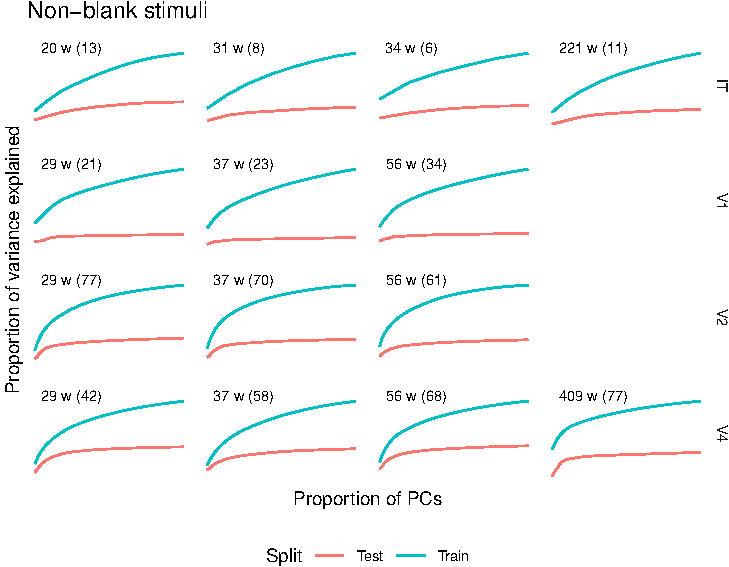
\includegraphics[keepaspectratio]{20260611_files/figure-pdf/fig-pca_nonblank-1.pdf}}

}

\caption{\label{fig-pca_nonblank}Comparisons between the variance
explained by the principal components for the training and test set,
organized by region (rows) and by session (columns). The proportion of
variance explained for the test set has been rescaled.}

\end{figure}%

\begin{figure}

\centering{

\pandocbounded{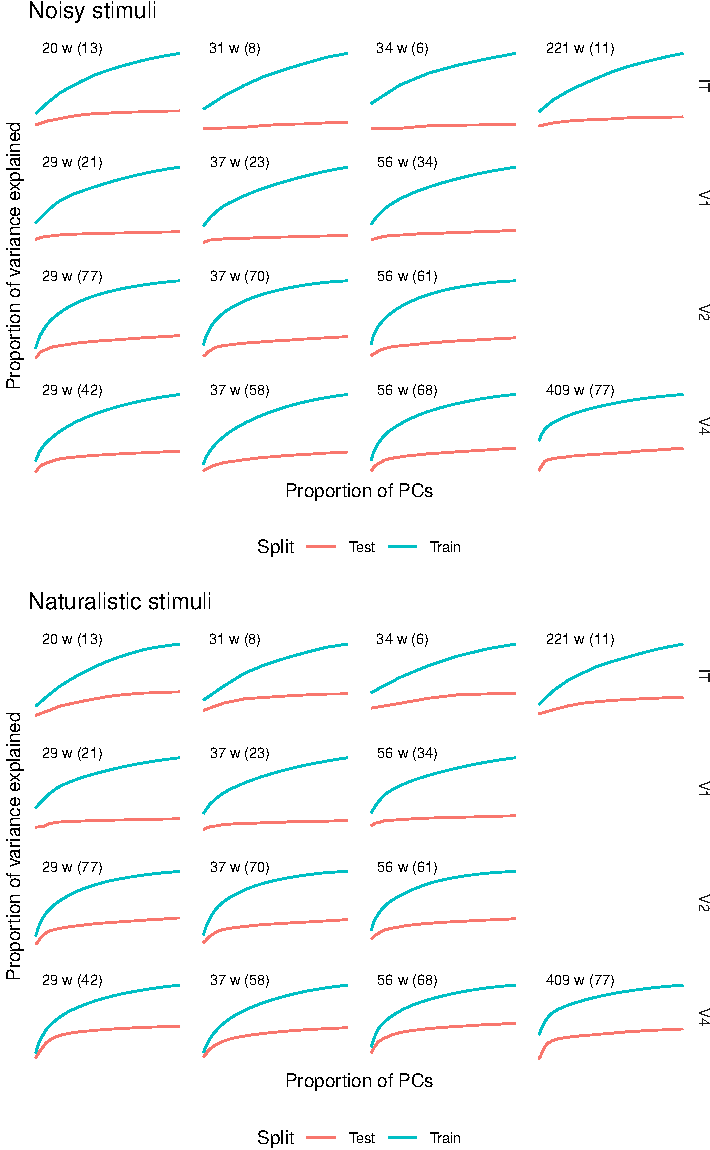
\includegraphics[keepaspectratio]{20260611_files/figure-pdf/fig-pca_coherence-1.pdf}}

}

\caption{\label{fig-pca_coherence}Same as previous figure, but noisy
stimuli are in the top section and naturalistic stimuli are in the
bottom.}

\end{figure}%

\begin{table}

\caption{\label{tbl-pca}Number of PCs to explain 90\% of the variance
(scaled to proportion for test set). Non-blank (NB), noisy (Ns),
naturalistic (Nt).}

\centering{

\fontsize{9.0pt}{11.0pt}\selectfont
\begin{tabular*}{\linewidth}{@{\extracolsep{\fill}}rrrrrrrr}
\toprule
Age (weeks) & Total PCs & Train (NB) & Train (Ns) & Train (Nt) & Test (NB) & Test (Ns) & Test (Nt) \\ 
\midrule\addlinespace[2.5pt]
\multicolumn{8}{l}{IT} \\[2.5pt] 
\midrule\addlinespace[2.5pt]
20 & 13 & 4 & 4 & 4 & 6 & 6 & 5 \\ 
31 & 8 & 2 & 2 & 2 & 4 & 2 & 4 \\ 
34 & 6 & 2 & 2 & 2 & 3 & 3 & 3 \\ 
221 & 11 & 3 & 3 & 3 & 5 & 5 & 5 \\ 
\midrule\addlinespace[2.5pt]
\multicolumn{8}{l}{V1} \\[2.5pt] 
\midrule\addlinespace[2.5pt]
29 & 21 & 7 & 6 & 8 & 15 & 9 & 13 \\ 
37 & 23 & 7 & 6 & 7 & 12 & 7 & 10 \\ 
56 & 34 & 10 & 10 & 11 & 23 & 11 & 19 \\ 
\midrule\addlinespace[2.5pt]
\multicolumn{8}{l}{V2} \\[2.5pt] 
\midrule\addlinespace[2.5pt]
29 & 77 & 32 & 31 & 34 & 40 & 20 & 27 \\ 
37 & 70 & 31 & 31 & 33 & 42 & 19 & 26 \\ 
56 & 61 & 28 & 27 & 30 & 33 & 17 & 28 \\ 
\midrule\addlinespace[2.5pt]
\multicolumn{8}{l}{V4} \\[2.5pt] 
\midrule\addlinespace[2.5pt]
29 & 42 & 15 & 13 & 16 & 27 & 14 & 23 \\ 
37 & 58 & 19 & 18 & 20 & 31 & 16 & 25 \\ 
56 & 68 & 27 & 25 & 28 & 42 & 19 & 34 \\ 
409 & 77 & 34 & 34 & 36 & 48 & 23 & 34 \\ 
\bottomrule
\end{tabular*}

}

\end{table}%

\section{Next steps}\label{next-steps}

\begin{itemize}
\tightlist
\item
  Running the above with a lower responsive channel threshold or with
  all channels regardless of responsiveness
\item
  Contrasting the early/late response (averaged over the first 70 ms
  vs.~the next 70 ms after onset) instead of over 150 ms after stimulus
  onset.
\end{itemize}




\end{document}
